% Quantitative measure of the force model
% Compile: xelatex quantitative_measure.tex  -> ../Force_model/Quantitative measure/quantitative_measure.pdf
\documentclass[11pt]{article}
\usepackage[a4paper,margin=2.5cm]{geometry}
\usepackage{amsmath,amssymb}
\usepackage{xeCJK}
\usepackage{tikz}
\usetikzlibrary{arrows.meta}
\setCJKmainfont[AutoFakeBold=2.5]{DFKai-SB}   % 標楷體
\setlength{\parindent}{0pt}

% Typography: vectors and matrices upright bold (\mathbf), scalars italic, not bold.
% Norms are written without the subscript 2.
\newcommand{\rh}{\hat{\mathbf{r}}}
\newcommand{\xa}{\hat{\mathbf{x}}_a}
\newcommand{\ya}{\hat{\mathbf{y}}_a}
\newcommand{\za}{\hat{\mathbf{z}}_a}
\newcommand{\Ij}{\mathbf{I}_j}
\newcommand{\Ijh}{\hat{\mathbf{I}}_j}
\newcommand{\fij}{\mathbf{f}_{ij}}

\begin{document}

\begin{center}
{\LARGE\bfseries Quantitative measure of the force model}
\end{center}
\vspace{6pt}

% ---------------------------------------------------------------------------------------
\section*{步驟 1}

\subsection*{1.1\ \ 單位方向 $\rh(\theta,\varphi)$}

以致動座標系的基底 $\{\xa,\ \ya,\ \za\}$ 描述任意單位方向 $\rh$：

\begin{minipage}[c]{0.54\textwidth}
\[
\rh(\theta,\varphi)
=\cos\varphi\cos\theta\,\xa+\cos\varphi\sin\theta\,\ya+\sin\varphi\,\za
=\begin{bmatrix}
\cos\varphi\cos\theta\\
\cos\varphi\sin\theta\\
\sin\varphi
\end{bmatrix}
\]
\[
\left\{
\begin{aligned}
\varphi &\in [-90^\circ,\ 90^\circ] &&\text{仰角（自 $x_a$--$y_a$ 平面起算）}\\
\theta  &\in [0^\circ,\ 360^\circ)  &&\text{方位角（自 $+x_a$ 軸起算，繞 $z_a$）}
\end{aligned}\right.
\]
\[
\|\rh\|=1
\]
\end{minipage}
\hfill
\begin{minipage}[c]{0.42\textwidth}
\centering
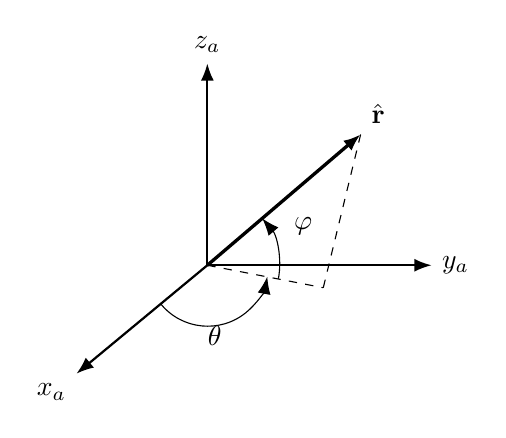
\begin{tikzpicture}[scale=0.95,>={Latex[length=2.2mm]}]
  \coordinate (O) at (0,0);
  \draw[->,thick] (O) -- (0,2.7)        node[above]{$z_a$};
  \draw[->,thick] (O) -- (3.0,0)        node[right]{$y_a$};
  \draw[->,thick] (O) -- (-1.75,-1.45)  node[below left]{$x_a$};
  \coordinate (V) at (2.05,1.75);
  \coordinate (Q) at (1.55,-0.30);
  \draw[->,very thick] (O) -- (V) node[above right]{$\rh$};
  \draw[dashed] (O) -- (Q);
  \draw[dashed] (Q) -- (V);
  \draw[->] (0.95,-0.18) arc (-10.5:40.5:0.97);
  \node at (1.28,0.52) {$\varphi$};
  \draw[->] (-0.62,-0.52) arc (219.5:349.5:0.81);
  \node at (0.10,-0.95) {$\theta$};
\end{tikzpicture}
\end{minipage}

\subsection*{1.2\ \ 電流 $\Ij$}

位置 $\mathbf{p}_i$、第 $j$ 組電流 $\Ij$ 產生的力向量
\[
\fij=\begin{bmatrix} f_{ij1}\\ f_{ij2}\\ f_{ij3} \end{bmatrix},\qquad
f_{ijk}=\Ij^{\mathsf T}\,{}^{F}\hat{\mathbf{H}}_{I}^{\mathsf T}\,
\mathbf{L}_k\!\left(\mathbf{p}_i/\hat{\ell},\,\hat{\mathbf{e}}\right)\,{}^{F}\hat{\mathbf{H}}_{I}\,\Ij,
\qquad k=1,2,3
\]
令
\[
\Ij=\sqrt{\|\fij\|}\;\Ijh,\qquad
\fij\!\left(\mathbf{p}_i,\Ij\right)=\|\fij\|\,\rh
\]
代入力模型：
\[
\begin{aligned}
\fij
&=\begin{bmatrix}
\left(\sqrt{\|\fij\|}\,\Ijh\right)^{\!\mathsf T}{}^{F}\hat{\mathbf{H}}_{I}^{\mathsf T}\,\mathbf{L}_1\!\left(\mathbf{p}_i/\hat{\ell},\hat{\mathbf{e}}\right){}^{F}\hat{\mathbf{H}}_{I}\left(\sqrt{\|\fij\|}\,\Ijh\right)\\[2pt]
\left(\sqrt{\|\fij\|}\,\Ijh\right)^{\!\mathsf T}{}^{F}\hat{\mathbf{H}}_{I}^{\mathsf T}\,\mathbf{L}_2\!\left(\mathbf{p}_i/\hat{\ell},\hat{\mathbf{e}}\right){}^{F}\hat{\mathbf{H}}_{I}\left(\sqrt{\|\fij\|}\,\Ijh\right)\\[2pt]
\left(\sqrt{\|\fij\|}\,\Ijh\right)^{\!\mathsf T}{}^{F}\hat{\mathbf{H}}_{I}^{\mathsf T}\,\mathbf{L}_3\!\left(\mathbf{p}_i/\hat{\ell},\hat{\mathbf{e}}\right){}^{F}\hat{\mathbf{H}}_{I}\left(\sqrt{\|\fij\|}\,\Ijh\right)
\end{bmatrix}\\[6pt]
&=\|\fij\|
\begin{bmatrix}
\Ijh^{\mathsf T}\,{}^{F}\hat{\mathbf{H}}_{I}^{\mathsf T}\,\mathbf{L}_1\!\left(\mathbf{p}_i/\hat{\ell},\hat{\mathbf{e}}\right){}^{F}\hat{\mathbf{H}}_{I}\,\Ijh\\[2pt]
\Ijh^{\mathsf T}\,{}^{F}\hat{\mathbf{H}}_{I}^{\mathsf T}\,\mathbf{L}_2\!\left(\mathbf{p}_i/\hat{\ell},\hat{\mathbf{e}}\right){}^{F}\hat{\mathbf{H}}_{I}\,\Ijh\\[2pt]
\Ijh^{\mathsf T}\,{}^{F}\hat{\mathbf{H}}_{I}^{\mathsf T}\,\mathbf{L}_3\!\left(\mathbf{p}_i/\hat{\ell},\hat{\mathbf{e}}\right){}^{F}\hat{\mathbf{H}}_{I}\,\Ijh
\end{bmatrix}\\[6pt]
&=\|\fij\|\;\hat{\mathbf{f}}_{ij}\!\left(\mathbf{p}_i,\Ijh\right)
\end{aligned}
\]
比較得
\[
\hat{\mathbf{f}}_{ij}\!\left(\mathbf{p}_i,\Ijh\right)=\rh
\]
$\hat{\mathbf{f}}_{ij}(\mathbf{p}_i,\Ijh)$ 稱為單位力量，所對應的電流 $\Ijh$ 稱為單位電流。

% ---------------------------------------------------------------------------------------
\section*{步驟 2}

期望力 $\mathbf{f}_d$ 拆成大小與方向：
\[
\mathbf{f}_d=\|\mathbf{f}_d\|\,\rh(\theta,\varphi)
\]
\[
\mathbf{I}_{\mathrm{opt}}=\arg\min_{\Ij}\ \|\Ij\|^2
\qquad\text{s.t.}\quad \fij\!\left(\mathbf{p}_i,\Ij\right)=\mathbf{f}_d
\]
以 $\Ij=\sqrt{\|\fij\|}\;\Ijh$ 替換 $\Ij$：
\[
\|\Ij\|^2=\|\fij\|\,\|\Ijh\|^2,\qquad
\fij\!\left(\mathbf{p}_i,\Ij\right)=\|\fij\|\,\hat{\mathbf{f}}_{ij}\!\left(\mathbf{p}_i,\Ijh\right)=\mathbf{f}_d
\]
限制式給出 $\|\fij\|=\|\mathbf{f}_d\|$、$\hat{\mathbf{f}}_{ij}(\mathbf{p}_i,\Ijh)=\mathbf{f}_d/\|\mathbf{f}_d\|=\rh$，$\|\mathbf{f}_d\|$ 為常數。\\[4pt]
換成最小範數單位電流問題：
\[
\hat{\mathbf{I}}_{\mathrm{opt}}(\varphi,\theta,\mathbf{p}_i)=\arg\min_{\Ijh}\ \|\Ijh\|^2
\qquad\text{s.t.}\quad \hat{\mathbf{f}}_{ij}\!\left(\mathbf{p}_i,\Ijh\right)=\rh
\]
原問題的解：
\[
\mathbf{I}_{\mathrm{opt}}=\sqrt{\|\mathbf{f}_d\|}\;\hat{\mathbf{I}}_{\mathrm{opt}}(\varphi,\theta,\mathbf{p}_i)
\]

% ---------------------------------------------------------------------------------------
\section*{步驟 3}

固定位置 $\mathbf{p}_i$，以 Lagrange multipliers 求解任意方向 $\rh$ 的 $\hat{\mathbf{I}}_{\mathrm{opt}}(\varphi,\theta,\mathbf{p}_i)$。令
\[
\mathbf{Q}_k={}^{F}\hat{\mathbf{H}}_{I}^{\mathsf T}\,\mathbf{L}_k\!\left(\mathbf{p}_i/\hat{\ell},\hat{\mathbf{e}}\right){}^{F}\hat{\mathbf{H}}_{I},
\qquad k=1,2,3
\]
限制式 $\hat{\mathbf{f}}_{ij}(\mathbf{p}_i,\Ijh)=\rh$ 的第 $k$ 個分量為 $\Ijh^{\mathsf T}\mathbf{Q}_k\Ijh=r_k$，
Lagrange multipliers $\boldsymbol{\lambda}=\begin{bmatrix}\lambda_1 & \lambda_2 & \lambda_3\end{bmatrix}^{\mathsf T}$：
\[
\mathcal{L}\!\left(\Ijh,\boldsymbol{\lambda}\right)
=\|\Ijh\|^2-\sum_{k=1}^{3}\lambda_k\left(\Ijh^{\mathsf T}\mathbf{Q}_k\Ijh-r_k\right)
\]

% ---------------------------------------------------------------------------------------
\section*{步驟 4}

限制電流大小 $\|\Ij\|\le\|\mathbf{I}\|_{\max}$。由 $\Ij=\sqrt{\|\fij\|}\;\Ijh$：
\[
\|\Ij\|^2=\|\fij\|\,\|\Ijh\|^2
\quad\Longrightarrow\quad
\|\fij\|=\frac{\|\Ij\|^2}{\|\Ijh\|^2}
\]
代回 $\fij=\|\fij\|\,\rh$：
\[
\fij=\frac{\|\Ij\|^2}{\|\Ijh\|^2}\,\rh
\]
方向 $\rh$ 固定時，取 $\|\Ij\|=\|\mathbf{I}\|_{\max}$、$\Ijh=\hat{\mathbf{I}}_{\mathrm{opt}}(\varphi,\theta,\mathbf{p}_i)$：
\[
\mathbf{f}_{ij,\max}\!\left(\mathbf{p}_i,\varphi,\theta,I_{\max}\right)
=\frac{\|\mathbf{I}\|_{\max}^2}{\left\|\hat{\mathbf{I}}_{\mathrm{opt}}(\varphi,\theta,\mathbf{p}_i)\right\|^2}\,\rh
\]
$\mathbf{f}_{ij,\max}$ 為位置 $\mathbf{p}_i$、電流大小不超過 $\|\mathbf{I}\|_{\max}$ 時，沿方向 $\rh(\theta,\varphi)$ 所能產生的最大力量。

% ---------------------------------------------------------------------------------------
\section*{步驟 5}

定義
\[
\rho\!\left(\mathbf{p}_i,\rh\right)=\frac{\left\|\hat{\mathbf{f}}_{ij}\right\|}{\left\|\hat{\mathbf{I}}_{\mathrm{opt}}\right\|^2}
\qquad(\mathrm{pN/A^2})
\]

% ---------------------------------------------------------------------------------------
\section*{步驟 6}

\[
\mathrm{capacity}(\mathbf{p}_i)
=\left(\frac{1}{4\pi}\int_{-\pi/2}^{\pi/2}\int_{0}^{2\pi}\rho^3\!\left(\mathbf{p}_i,\rh\right)\cos\varphi\;d\theta\,d\varphi\right)^{1/3}
\qquad(\mathrm{pN/A^2})
\]
\[
\mathrm{isotropy}(\mathbf{p}_i)
=\frac{\displaystyle\min_{\rh}\ \rho\!\left(\mathbf{p}_i,\rh\right)}{\displaystyle\max_{\rh}\ \rho\!\left(\mathbf{p}_i,\rh\right)}
\]

\end{document}
